L'application de nos algorithmes de d\'ecouverte et de correction d\'ebute par la g\'en\'eration de $500$ topologies \'electriques $G$ de $30$ sommets, chacune ayant un degr\'e maximal moyen de  $\Delta(G) = 5$.
Nous construisons $500$ line-graphes $LG$ de $150$ sommets et $470$ ar\^etes, en moyenne. \newline
Nous avons donc introduit trois param\`etres $k, p,  \alpha_{max}$:
\begin{enumerate}
\item Le param\`etre $k$ d\'esigne le nombre de cases modifi\'ees dans la matrice $M_{LG}$. Dans notre \'etude, $k \in \{1,\cdots,9\}$.
\item Le param\`etre $p$ d\'esigne la proportion de cases \`a $0$ s\'electionn\'ees parmi les $k$ cases. Dans notre \'etude, $p \in \{0.1,\cdots,0.9\}$.
\item Le param\`etre $\alpha_{max}$ d\'esigne le nombre de graphes g\'en\'er\'es pour un couple  $(k, p)$ de valeurs donn\'ees.
%\item Le param\`etre $\alpha = \{1,\cdots, \alpha_{max} \}$ d\'esigne le nombre de fois qu'on modifie $k$ cases dans la  matrice $M_{LG}$ pour une valeur de $p$ donn\'ee. Il est utilis\'e pour faire varier les $k$ cases choisies dans un graphe. 
\end{enumerate}
 
Nous  choisissons $\alpha_{max} = 5$ pour des temps de calculs r\'ealistes. 
Chaque graphe g\'en\'er\'e est identifi\'e par une valeur de  $\alpha \in \{1,\cdots, \alpha_{max} \}$, est not\'e $G_{k,p,\alpha}$ et sa matrice d'adjacence est  $M_{k,p,\alpha}$. 
La valeur $\alpha$ d\'esigne l'indice de modification de $k$ cases dans la  matrice $M_{LG}$ pour une valeur de $p$ donn\'ee. Il est utilis\'e pour faire varier les $k$ cases choisies dans un graphe. 
Nous appliquons notre couple d'algorithmes sur une matrice $M_{k,p,\alpha}$ et nous obtenons la matrice $M'_{k,p,\alpha}$ qui est la matrice d'adjacence du line-graphe $LG_{k, p, \alpha}$. 

% a ajouter des distance line et hamming
Pour comparer les ar\^etes entre les graphes $LG_{k,p, \alpha}$ et $G_{k,p, \alpha}$, nous calculons la distance de correction (section \ref{algorithmeCorrection}) not\'ee $DC_{k,p, \alpha}$.
De m\^eme, le nombre d'ar\^etes diff\'erentes entre les graphes $LG_{k,p, \alpha}$ et $LG$ d\'efinit la distance de Hamming $DH_{k,p, \alpha}$.
Nous d\'efinissons par les variables $moy\_DH_{k,p}$ et $moy\_DC_{k,p}$, les moyennes respectives des distances de Hamming (not\'ee $DH_{k,p,\alpha}$) et des distances de correction (not\'ee $DC_{k,p,\alpha}$) pour une valeur donn\'ee de $k$ et pour tout $\alpha \in \{1, \cdots, \alpha_{max}\}$.
\begin{equation}
moy\_DH_{k, p} = \sum_{\alpha = 1}^{ \alpha_{max} } DH_{k, p, \alpha} \hspace{1 em}; 
moy\_DC_{k, p} = \sum_{\alpha = 1}^{ \alpha_{max} } DC_{k, p, \alpha}
\end{equation}

Les diff\'erentes \'etapes de l'exp\'erimentation sont r\'esum\'ees dans la figure \ref{recapProtocoleEtude}. Les \'etapes sont repr\'esent\'ees par des graphes et les phases de modification de ces graphes sont d\'esign\'ees par les fl\`eches unidirectionnelles. Quant aux fl\`eches bidirectionnelles (en rouge), elles indiquent le calcul de distances (de Hamming et de correction). 
% ------------  figure recap Protocole Etude  ----------------------
\begin{figure}[htb!] 
\centering
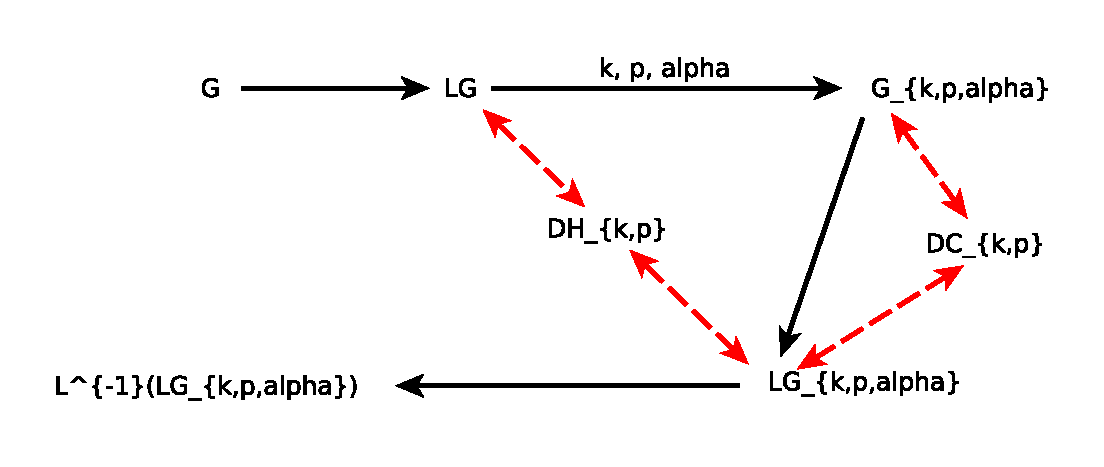
\includegraphics[scale=0.750]{recapProtocoleEtude.eps}
\caption{\'Etapes de l'exp\'erimentation :  \\
1) On g\'en\`ere le graphe $G$ et son line-graphe $LG$;\\ 
2) On modifie $k$ cases la $\alpha^{ieme}$ fois selon la repartition $p$ pour obtenir le graphe $G_{k,p,\alpha}$;\\ 
3) On applique les algorithmes de couverture et de correction pour avoir un line-graphe $LG_{k,p,\alpha}$. $LG_{k,p,\alpha}$ et  $G_{k,p,\alpha}$ diff\`erent de $DC_{k,p,\alpha}$ ar\^etes. $LG_{k,p,\alpha}$ a $DH_{k,p,\alpha}$ cases modifi\'ees par rapport \`a $LG$; 
\\ 4) $L^{-1}(LG_{k,p,\alpha})$ est le graphe racine de $LG_{k,p,\alpha}$. }
\label{recapProtocoleEtude} 
\end{figure}
% ------------  figure recap Protocole Etude  ----------------------
%\FloatBarrier
\newline


% correction du graphe
% 1) comment je selectionne (choisis) les sommets -1
%		- remise: on selectionne un sommet de sommets -1 selon une methode puis on la corrige. Ensuite, on applique notre couple d'algorithme  sur le graphe corrig\'e. On reprend l'operation tant que graphe corrige n'est pas un line-graphe    
%		- sans remise: On choisit une permutation des sommets de sommets-1 puis on les corrige les uns a la suite des autres.Les sommets dans la permutation sont ordonnee selon  la methode suivante:
% 		* degre min : les sommets sont ranges par ordre croissant de leur degre.
%		* cout min : les sommets sont ranges par ordre croissant de leur cout. Le cout est la somme du poids de chaque case modifi\'e.
%		* aleatoire :  les sommets sont ranges sans condition prealable.
%			* aleatoire * cout min * degre min
%correction
Soit ${\cal C}$ l'ensemble des sommets n'\'etant couverts par aucune clique apr\`es l'algorithme de couverture.
La correction de la matrice $M_{k,p,\alpha}$ est n\'ecessaire s'il existe des sommets appartenant \`a ${\cal C}$. 
\newline
Nous distinguons deux modes d'ex\'ecution de notre algorithme de correction:
\begin{enumerate}
	\item Mode avec remise :
%			\begin{algorithm}[!ht]
				\newline
				\noindent 1. Ex\'ecution algorithme de couverture, {\bf return} ${\cal C}$ \\
				~2. \indent {\bf Tant que} ${\cal C}$ n'est pas vide\\ 
				~3.	       	\indent~~~~~~~~Correction d'un sommet de ${\cal C}$  \\
				~4.	       	\indent~~~~~~~~Ex\'ecution algorithme de couverture, {\bf return} ${\cal C}$ \\
%			\end{algorithm}
	\item Modes sans remise :
%			\begin{algorithm}[!ht]
				\newline
				\noindent 1. Ex\'ecution algorithme de couverture, {\bf return} ${\cal C}$ \\
				~2. \indent {\bf Tant que} ${\cal C}$ n'est pas vide\\ 
				~3.	       	\indent~~~~~~~~Correction d'un sommet de ${\cal C}$  \\
				~4.	       	\indent~~~~~~~~Mise \`a jour du sommet  de ${\cal C}$  \\
%			\end{algorithm}
\end{enumerate}
\`A chaque \'etape $3$ dans les deux modes, un sommet de $\cal C$ est choisi selon :
\begin{enumerate} [label = (\alph*)]
\item {\em Degr\'e minimum} : le sommet de degr\'e minimum est s\'electionn\'e. 
\item {\em Co\^ut minimum} : le sommet de  co\^ut de compression minimum est s\'electionn\'e. Le co\^ut de compression est la somme des co\^uts de chaque case modifi\'ee. 
\item {\em Al\'eatoire} : le sommet est s\'electionn\'e al\'eatoirement parmi les sommets de $\cal C$.
\end{enumerate}
La correction de chaque sommet de ${\cal C}$ implique l'ajout et la suppression des ar\^etes du graphe. Nous souhaitons orienter les d\'ecisions de l'algorithme de correction de telle sorte qu'il ajoute  ou supprime uniquement des ar\^etes ou 
qu'il r\'ealise les deux op\'erations.
%que la correction d'un sommet s'effectue soit en ajoutant des ar\^etes, soit en supprimant des ar\^etes ou  soit en r\'ealisant les deux op\'erations. 
 Nous  priorisons une op\'eration en attribuant des co\^uts diff\'erents \`a  la modification d'ar\^etes.
Nous distinguons trois types d'op\'erations que nous appelons {\em fonctions de co\^ut} :
\begin{enumerate}[label=(\roman*)]
\item {\em Unitaire} : l'ajout et la suppression d'une ar\^ete ont un m\^eme co\^ut c'est-\`a-dire $1$.
\item {\em Ajout} : l'ajout d'une ar\^ete a un co\^ut de $1$ et la suppression a un co\^ut de $2$.
\item {\em Suppression} : l'ajout d'une ar\^ete a un co\^ut de $2$ et la suppression a un co\^ut de $1$.
\end{enumerate}
Nous rappelons que la distance de correction n'est pas la somme de toutes les  modifications d'ar\^etes r\'ealis\'ees. En effet, une ar\^ete  supprim\'ee et ajout\'ee plusieurs fois (pour diff\'erents sommets de ${\cal C}$) n'est comptabilis\'ee qu'une fois et son co\^ut est appliqu\'e selon la fonction de co\^ut.
\newline


\'Etant donn\'ee que nous avons $3$ fonctions de co\^ut, $2$ modes de correction et $3$  s\'elections possibles des sommets, nous nous retrouvons avec $18$ approches de correction de sommets et il est fastidieux de les interpr\'eter sur une m\^eme figure.
Ainsi nous nous limitons \`a la fonction de co\^ut {\em unitaire} dans un premier temps et nous consid\'erons les approches de correction suivantes : $1a$, $1b$, $2a$, $2b$, $2c$.  
La lecture de l'approche de correction $(1a)$ est le suivant : $1)$ avec remise et $a)$ le degr\'e minimum.
L'approche $(1c)$ n'est d'aucune utilit\'e car l'algorithme de correction ne parvient pas \`a fournir un line-graphe. En effet, l'ensemble $\cal C$ croit lin\'eairement \`a chaque \'etape de correction et la correction devient une boucle infinie.
%En effet, nous avons rencontr\'e des cas dans lesquels l'algorithme de correction est dans une boucle infinie parce que les sommets corrig\'es augmentent l'ensemble $\cal C$ et les cases modif\'ees par chaque sommet corrig\'e \'eloignent la matrice obtenue de celle d'un line-graphe.
Le tableau \ref{tab:recapApprocheCorrection} r\'esume les approches de correction retenues dans l'analyse des performances de l'algorithme de correction.
% ------------ tableau recapitulatif -----------------------
%\begin{table}[h]
%   \centering
%   \caption{\label{tab:recapApprocheCorrection} tableau r\'ecapitulatif des approches de corrections }
%   \begin{tabular}{|l|c|c|r|}
%   	\hline
%  	Mode & choix sommets & fonction de co\^ut & paragraphes \\
%  	\hline
%%  	Sans Remise & Degre Min & unitaire & 1  \\
%%  	\cline{1-9}     & \cline{1-3} & ajout       & 1  \\
%	\multirow{9}{*}{Sans r\'emise} & 
%								\multirow{3}{*}{degr\'e minimum} & unitaire & x\\
%															  & & ajout & y\\
%															  & & suppression & z\\
%															  \hline
%							& 
%								\multirow{3}{*}{co\^ut minimum} & unitaire & x\\
%															  & & ajout & y\\
%															  & & suppression & z\\
%															  \hline								  
%							& 
%								\multirow{3}{*}{al\'eatoire} & unitaire & x\\
%															  & & ajout & y\\
%															  & & suppression & z\\
%															  \hline
%															  \hline									 
%	\multirow{6}{*}{Avec r\'emise} & 
%								\multirow{3}{*}{degr\'e minimum} & unitaire & x\\
%															  & & ajout & y\\
%															  & & suppression & z\\
%															  \hline
%							& 
%								\multirow{3}{*}{co\^ut minimum} & unitaire & x\\
%															  & & ajout & y\\
%															  & & suppression & z\\
%															  \hline															  
%   \end{tabular}
%\end{table}
\begin{table}[h]
   \centering
   \caption{\label{tab:recapApprocheCorrection} Tableau r\'ecapitulatif des approches de corrections }
   \begin{tabular}{|l|c|c|r|}
   	\hline
  	Mode & choix sommets & fonction de co\^ut  \\
  	\hline
%  	Sans Remise & Degre Min & unitaire & 1  \\
%  	\cline{1-9}     & \cline{1-3} & ajout       & 1  \\
	 & 
								\multirow{3}{*}{degr\'e minimum} & unitaire \\
															  & & ajout \\
									
												& & suppression \\
											
								\cline{2-3}
	Sans remise						& 
								\multirow{3}{*}{co\^ut minimum} & unitaire \\
															  & & ajout \\
															  & & suppression \\
															  \cline{2-3}								  
							& 
								\multirow{3}{*}{al\'eatoire} & unitaire \\
															  & & ajout \\
															  & & suppression \\
															  \hline
															  \hline									 
	 & 
								\multirow{3}{*}{degr\'e minimum} & unitaire \\
															  & & ajout \\
															  & & suppression \\
															 \cline{2-3}
	Avec remise						& 
								\multirow{3}{*}{co\^ut minimum} & unitaire \\
															  & & ajout \\
															  & & suppression \\
															  \hline															  
   \end{tabular}
\end{table}
% ------------ tableau recapitulatif -----------------------
\newline

Nous recherchons l'approche qui traite le probl\`eme {\em Proxi-Line} c'est-\`a-dire le mode qui majore la distance line de $G_{k,p}$ par la distance de correction entre $LG_{k,p}$ et $G_{k,p}$.
Une fois le meilleur mode trouv\'e, nous comparons les fonctions de co\^ut $i$, $2i$ et $3i$ avec ce mode pour trouver l'influence de la fonction de co\^ut sur les distances de correction.

%---- decription protocole d'etude --> fin